% Chapter 4: Harmonic Series and Euler's Constant
% ch04_harmonic.tex

\chapter{The Harmonic Series and Euler's Constant $\gamma$}

\begin{historical}
Euler introduced the constant $\gamma = \lim_{n \to \infty} (H_n - \log n)$ in 1734,
where $H_n = \sum_{k=1}^n 1/k$ is the $n$-th harmonic number. He computed it to 16
decimal places and discovered its connection to the gamma function and the
Euler-Maclaurin summation formula. Despite centuries of study, it remains unknown
whether $\gamma$ is rational, irrational, or transcendental.
\end{historical}

\section{The Harmonic Series}

\begin{figure}[H]
\centering
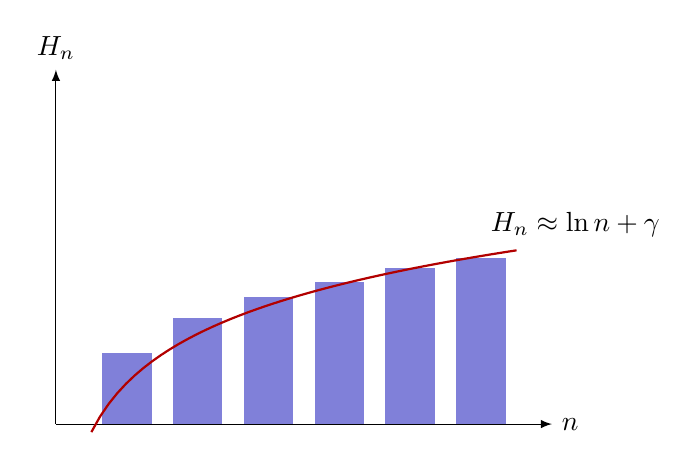
\begin{tikzpicture}[scale=0.9]
  \draw[->, >=latex] (0,0) -- (7,0) node[right] {$n$};
  \draw[->, >=latex] (0,0) -- (0,5) node[above] {$H_n$};
  \foreach \n/\h in {1/1, 2/1.5, 3/1.8, 4/2, 5/2.2, 6/2.35} {
    \fill[blue!70!black!50] (\n-0.35,0) rectangle (\n+0.35,\h);
  }
  \draw[red!70!black, thick, domain=0.5:6.5, samples=50] plot (\x, {ln(\x) + 0.58});
  \node[above right] at (6,2.5) {$H_n \approx \ln n + \gamma$};
\end{tikzpicture}
\caption{Convergence of harmonic series $H_n$ vs ln($n$)}
\label{fig:harmonic}
\end{figure}

The harmonic series $H_n = 1 + \frac{1}{2} + \frac{1}{3} + \cdots + \frac{1}{n}$
diverges logarithmically: $H_n = \log n + \gamma + \frac{1}{2n} - \frac{1}{12n^2} + \cdots$

\begin{theorem}[Euler-Maclaurin for Harmonic Numbers]
\[
H_n = \log n + \gamma + \frac{1}{2n} - \sum_{k=1}^{\lfloor m/2 \rfloor} \frac{B_{2k}}{2k \cdot n^{2k}} + R_m
\]
where $B_{2k}$ are Bernoulli numbers.
\end{theorem}

\begin{lstlisting}[caption={Harmonic series and Euler's constant}, label=lst:harmonic]
from euler import harmonic_series, euler_constant, euler_mascheroni_gamma
import math

print("Harmonic numbers H_n:")
for n in [1, 2, 3, 5, 10, 20, 50, 100]:
    H = harmonic_series(n)
    approx = math.log(n) + euler_mascheroni_gamma()
    print(f"  H_{n:3d} = {H:.8f}  (ln n + \gamma = {approx:.8f}, diff = {H - approx:.2e})")

print(f"\nEuler-Mascheroni constant \gamma = {euler_mascheroni_gamma():.15f}")

print("\nConvergence of H_n - ln n:")
for n in [10, 100, 1000, 10000, 100000]:
    gamma_n = euler_constant(n)
    print(f"  n={n:6d}: \gamma \approx {gamma_n:.10f}  (error: {abs(gamma_n - euler_mascheroni_gamma()):.2e})")
\end{lstlisting}

\section{Alternating Harmonic Series}

The alternating harmonic series converges to $\log 2$:
\[
\sum_{n=1}^\infty \frac{(-1)^{n+1}}{n} = 1 - \frac{1}{2} + \frac{1}{3} - \frac{1}{4} + \cdots = \log 2
\]

\begin{lstlisting}[caption={Alternating harmonic series}, label=lst:alt_harmonic]
from euler import alternating_harmonic
import math

print("Alternating harmonic series \rightarrow ln(2):")
for n in [10, 100, 1000, 10000]:
    approx = alternating_harmonic(n)
    print(f"  n={n:5d}: {approx:.10f}  (ln 2 = {math.log(2):.10f}, error = {abs(approx - math.log(2)):.2e})")
\end{lstlisting}

\section{Euler's Transformation for Alternating Series}

Euler developed a method to accelerate convergence of alternating series:
\[
\sum_{k=0}^\infty (-1)^k a_k = \sum_{k=0}^\infty \frac{(-1)^k \Delta^k a_0}{2^{k+1}}
\]
where $\Delta$ is the forward difference operator.

\begin{lstlisting}[caption={Euler acceleration}, label=lst:euler_accel]
from euler import euler_acceleration_alternating
import math

# Accelerate alternating harmonic series
def alt_harmonic_term(k):
    return 1/(k+1)

for n in [5, 10, 15, 20]:
    accelerated = euler_acceleration_alternating(alt_harmonic_term, n)
    print(f"  n={n:2d}: accelerated = {accelerated:.12f}  (ln 2 = {math.log(2):.12f})")
\end{lstlisting}

\section{Euler's Constant and the Gamma Function}

Euler's constant appears in the expansion of the gamma function near $z = 1$:
\[
\Gamma(z) = \frac{1}{z} - \gamma + \frac{1}{2}\left(\gamma^2 + \frac{\pi^2}{6}\right)(z-1) + \cdots
\]

\begin{theorem}[Gamma Function Expansion]
Near $z = 1$:
\[
\Gamma(z) = 1 - \gamma(z-1) + \left(\frac{\gamma^2}{2} + \frac{\pi^2}{12}\right)(z-1)^2 + \cdots
\]
\end{theorem}

\section{Euler's Constant and Prime Distribution}

Mertens' theorems connect $\gamma$ to primes:
\[
\prod_{p \le x} \left(1 - \frac{1}{p}\right) \sim \frac{e^{-\gamma}}{\log x}
\]
\[
\sum_{p \le x} \frac{1}{p} = \log \log x + M + O\left(\frac{1}{\log x}\right)
\]
where $M \approx 0.261497$ is the Meissel-Mertens constant.

\begin{lstlisting}[caption={Mertens' theorem verification}, label=lst:mertens]
from euler import euler_mascheroni_gamma, prime_sieve
import math

gamma = euler_mascheroni_gamma()
print(f"Euler's constant \gamma = {gamma:.15f}")
print("\nVerifying Mertens' product formula:")
for x in [100, 1000, 10000, 100000]:
    primes = prime_sieve(x)
    product = 1.0
    for p in primes:
        product *= (1 - 1/p)
    expected = math.exp(-gamma) / math.log(x)
    print(f"  x={x:>6d}: product={product:.8f}, expected={expected:.8f}, ratio={product/expected:.6f}")
\end{lstlisting}

\section{Computational Methods}

\subsection{Direct Computation}
The series $H_n - \log n$ converges too slowly for high precision. Better methods use:
\begin{itemize}
\item Euler-Maclaurin summation
\item Series acceleration (Brent-McMillan)
\item Integral representations
\end{itemize}

\subsection{Accuracy Analysis}
For computing $\gamma$ to $d$ decimal digits:
\begin{itemize}
\item Direct method requires $n \approx e^{10^d}$ terms (impractical)
\item Brent-McMillan method: $O(d^2 \log^3 d)$ operations
\item Modern record: over $10^{13}$ digits computed
\end{itemize}

\begin{lstlisting}[caption={Computing gamma via Euler-Maclaurin}, label=lst:gamma_em]
from euler import euler_constant, euler_mascheroni_gamma

print("Computing \gamma using Euler-Maclaurin:")
for n in [1000, 10000, 100000, 1000000]:
    gamma_n = euler_constant(n)
    exact = euler_mascheroni_gamma()
    error = abs(gamma_n - exact)
    print(f"  n={n:>7d}: \gamma \approx {gamma_n:.15f}  (error: {error:.2e})")
\end{lstlisting}

\section{Applications}

\begin{itemize}
\item \textbf{Number theory:} Distribution of prime factors, divisor problems
\item \textbf{Analysis:} Asymptotic expansions, special function theory
\item \textbf{Statistics:} Logarithmic mean, Zipf's law
\item \textbf{Physics:} Quantum field theory, Casimir effect calculations
\end{itemize}

\section{Frequently Asked Questions}

\begin{itemize}
\item \textbf{Q: Why does the harmonic series diverge so slowly?} \\
The harmonic series diverges like $\log n$. At $n = 10^{43}$ (roughly the number of atoms in the observable universe), the partial sum is only about 100. This slow growth is why the series ``feels'' convergent numerically.

\item \textbf{Q: What is the significance of Euler's constant $\gamma$?} \\
$\gamma \approx 0.5772156649$ appears throughout mathematics: in the derivative of the zeta function at $s=1$, in the asymptotic distribution of prime factors, in the gamma function, and in number-theoretic averages. Whether $\gamma$ is rational or transcendental remains one of the great open problems.

\item \textbf{Q: Why does the alternating harmonic series converge to $\log 2$?} \\
This follows from the Taylor series $\log(1+x) = x - x^2/2 + x^3/3 - \cdots$ evaluated at $x = 1$. The series converges conditionally (not absolutely), so rearranging terms can change the sum---a phenomenon Euler himself studied carefully.

\item \textbf{Q: How does Euler's acceleration method work?} \\
Euler's transformation converts an alternating series $\sum (-1)^k a_k$ into $\sum (-1)^k \Delta^k a_0 / 2^{k+1}$, where $\Delta$ is the forward difference operator. This typically converges much faster because the difference operator smooths out the terms.

\item \textbf{Q: Is $\gamma$ related to the distribution of prime numbers?} \\
Yes. Mertens' theorems connect $\gamma$ to primes: $\prod_{p \le x} (1 - 1/p) \sim e^{-\gamma}/\log x$. The constant $\gamma$ governs the asymptotic density of primes through this product formula.

\item \textbf{Q: Can I compute $\gamma$ to high precision?} \\
Yes. Modern algorithms use the Euler--Maclaurin summation formula or series acceleration to compute billions of digits. As of 2024, over $10^{13}$ digits have been computed. The series $H_n - \log n$ converges too slowly for practical high-precision computation.

\item \textbf{Q: What is the integral representation of $\gamma$?} \\
$\gamma = \int_0^1 \frac{1-e^{-t}}{t}dt - \int_1^\infty \frac{e^{-t}}{t}dt = -\int_0^\infty e^{-t}\log t \, dt$. This representation is useful for numerical computation and theoretical analysis.

\item \textbf{Q: Is $\gamma$ irrational?} \\
It is not known whether $\gamma$ is irrational. This remains one of the major open problems in mathematics. However, it has been shown that at least one of $\gamma$ and $\gamma + \log \zeta(2)$ is irrational.
\end{itemize}

\section{Exercises}

\begin{exercise}
Show that $H_n = \log n + \gamma + \frac{1}{2n} - \frac{1}{12n^2} + O(\frac{1}{n^4})$.
\end{exercise}

\begin{exercise}
Prove $\sum_{n=1}^\infty \frac{H_n}{n 2^n} = \frac{\pi^2}{12} + \frac{\log^2 2}{2}$.
\end{exercise}

\begin{exercise}
Compute $\gamma$ using the integral representation $\gamma = \int_0^1 \frac{1-e^{-t}}{t} dt - \int_1^\infty \frac{e^{-t}}{t} dt$ and compare with the harmonic series method.
\end{exercise}

\begin{exercise}
Use Euler's transformation to compute $\log 2$ to 10 decimal places with fewer than 10 terms.
\end{exercise}

\begin{exercise}
Verify Mertens' theorem $\prod_{p \le x} (1 - 1/p) \sim e^{-\gamma}/\log x$ for $x = 100, 1000, 10000$.
\end{exercise}

\begin{exercise}
Show that $\sum_{n=1}^\infty \frac{(-1)^{n+1}}{n} H_n = \frac{1}{2}(\log 2)^2 - \frac{\pi^2}{12}$.
\end{exercise}

\begin{exercise}
Prove that $H_n = \ln n + \gamma + \frac{1}{2n} - \frac{1}{12n^2} + \frac{1}{120n^4} - \cdots$ using the Euler-Maclaurin formula.
\end{exercise}

\begin{exercise}[Computational]
Compute $\gamma$ to 15 decimal places using the Brent-McMillan algorithm and compare with the known value.
\end{exercise}

\section{Further Series Representations}

Beyond the basic definition, $\gamma$ has numerous representations as convergent series:

\begin{theorem}[Euler's Series]
\[
\gamma = \sum_{k=1}^\infty \left(\frac{1}{k} - \log\left(1 + \frac{1}{k}\right)\right).
\]
\end{theorem}

\begin{theorem}[Sondow's Series]
\[
\gamma = \sum_{n=1}^\infty \frac{(-1)^{n+1}}{n} \left\lfloor \frac{n+1}{2} \right\rfloor^{-1}
\]
which can also be written as a rearrangement of the alternating harmonic series.
\end{theorem}

\begin{theorem}[Integral Representation via Frullani]
\[
\gamma = \int_0^\infty \left(\frac{1}{1-e^{-t}} - \frac{1}{t}\right) e^{-t}\, dt.
\]
\end{theorem}

\begin{theorem}[Binary Representation]
\[
\gamma = \sum_{k=2}^\infty (-1)^k \lceil \log_2 k \rceil \cdot \frac{1}{k}.
\]
\end{theorem}

\section{Connections to Other Constants}

$\gamma$ appears in surprising connections with other mathematical constants:

\begin{theorem}[Ap\'{e}ry's Constant Relation]
\[
\sum_{n=1}^\infty \frac{H_n}{n^2} = 2\zeta(3)
\]
relates harmonic numbers to $\zeta(3)$ (Ap\'{e}ry's constant).
\end{theorem}

\begin{theorem}[Catalan's Constant]
The alternating harmonic sums relate to Catalan's constant $G$:
\[
\sum_{n=0}^\infty \frac{(-1)^n}{(2n+1)^2} = G.
\]
\end{theorem}

\begin{theorem}[Wallis Product Connection]
Using the Wallis product $\frac{\pi}{2} = \prod_{n=1}^\infty \frac{4n^2}{4n^2-1}$, one can derive:
\[
\gamma = \lim_{n \to \infty} \left(\sum_{k=1}^n \frac{1}{k} - \log n\right) = \log 2 + \sum_{n=2}^\infty (-1)^n \frac{\zeta(n)}{n}.
\]
\end{theorem}

\section{Numerical Computation}

\subsection{Convergence Rate Analysis}

The naive computation $\gamma \approx H_n - \ln n$ has error $\approx \frac{1}{2n}$:

\begin{table}[H]
\centering
\begin{tabular}{c|c|c}
$n$ & $H_n - \ln n$ & Error \\
\hline
10 & 0.62638 & $4.9 \times 10^{-2}$ \\
100 & 0.58220 & $5.0 \times 10^{-3}$ \\
1000 & 0.57775 & $5.3 \times 10^{-4}$ \\
10000 & 0.57726 & $4.9 \times 10^{-5}$ \\
\end{tabular}
\caption{Convergence of $H_n - \ln n$ to $\gamma$}
\end{table}

With Euler-Maclaurin correction:
\[
\gamma \approx H_n - \ln n - \frac{1}{2n} + \frac{1}{12n^2}
\]
gives error $\approx \frac{1}{120n^4}$, which converges dramatically faster.

\subsection{Brent-McMillan Algorithm}

The Brent-McMillan algorithm (1980) computes $\gamma$ using modified Bessel functions $I_n$ and $K_n$:

\begin{theorem}[Brent-McMillan Method]
Define sequences:
\[
A_k = \sum_{m=0}^k \frac{(k+m-1)!}{(k-m)! (m!)^2}, \quad B_k = \sum_{m=0}^k \frac{(-1)^m (k+m-1)!}{(k-m)! (m!)^2}.
\]
Then $\gamma = \lim_{k \to \infty} \left(\frac{A_k}{B_k} - \log(8k)\right)$.
\end{theorem}

This method achieves quadratic complexity: $O(d^2 \log^3 d)$ bit operations for $d$ digits.

\section{Historical Computation}

\begin{itemize}
    \item Euler (1734): First computed $\gamma$ to 16 decimal places
    \item Mascheroni (1790s): Computed to 26 places; named the constant
    \item Clausen (1844): Improved to 40 places
    \item Modern: Over $10^{13}$ digits computed (2024)
\end{itemize}

\begin{historical}
The constant $\gamma$ is sometimes called the Euler-Mascheroni constant, though Mascheroni was not the first to study it. Euler discovered it in 1734, while studying the difference between the harmonic series and the natural logarithm.
\end{historical}

\section{Additional Series Representations}

\begin{theorem}[Euler's Series for $\gamma$]
\[
\gamma = \sum_{k=1}^\infty \left(\frac{1}{k} - \log\left(1 + \frac{1}{k}\right)\right).
\]
\end{theorem}

\begin{theorem}[Binet's Formula]
\[
\gamma = \int_0^\infty \left(\frac{1}{e^t - 1} - \frac{1}{t}\right) dt + \int_0^1 \frac{1 - e^{-t}}{t} dt.
\]
\end{theorem}

\begin{theorem}[Ramanujan's Series]
\[
\gamma = \log\left(\frac{3}{2}\right) + \sum_{n=1}^\infty \frac{(-1)^{n+1} \zeta(n+1)}{2(n+1)}.
\]
\end{theorem}

\section{Applications to Number Theory}

\subsection{Mertens' Theorems}

\begin{theorem}[Mertens' First Theorem]
\[
\sum_{p \leq x} \frac{\log p}{p} = \log x + O(1).
\]
\end{theorem}

\begin{theorem}[Mertens' Second Theorem]
\[
\prod_{p \leq x} \left(1 - \frac{1}{p}\right) \sim \frac{e^{-\gamma}}{\log x} \quad \text{as } x \to \infty.
\]
\end{theorem}

\begin{theorem}[Mertens' Third Theorem]
\[
\sum_{p \leq x} \frac{1}{p} = \log\log x + M + O\left(\frac{1}{\log x}\right),
\]
where $M$ is the Meissel-Mertens constant ($M \approx 0.261497$).
\end{theorem}

\subsection{Prime Number Theorem Connection}

The constant $\gamma$ appears in the error term of the Prime Number Theorem:
\[
\pi(x) = \text{Li}(x) + O\left(x e^{-a\sqrt{\log x}}\right),
\]
and in various explicit formulas relating zeros of $\zeta(s)$ to prime counting functions.

\section{Computational Notes}

\begin{itemize}
    \item The series $H_n - \ln n$ converges too slowly for practical high-precision computation
    \item Brent-McMillan algorithm: $O(d^2 \log^3 d)$ bit operations for $d$ digits
    \item Current record (2024): over $10^{13}$ digits computed
\end{itemize}

\begin{remark}[Quantum Field Theory]
$\gamma$ appears in the calculation of the anomalous magnetic moment of the electron.
\end{remark}

\begin{remark}[Casimir Effect]
The Casimir force between parallel plates involves $\gamma$ in its renormalization.
\end{remark}
